\section{Aufbau}
\label{sec:Aufbau}
Es wird eine Schaltung gemäß des in Abbildung \ref{fig:Aufbau} zu sehenden Schemas aufgebaut. Die als Probe verwendete $\beta$-Quelle wird auf der Seite des eingewölbten Mylar-Fensters positioniert. 
\begin{figure}
\centering
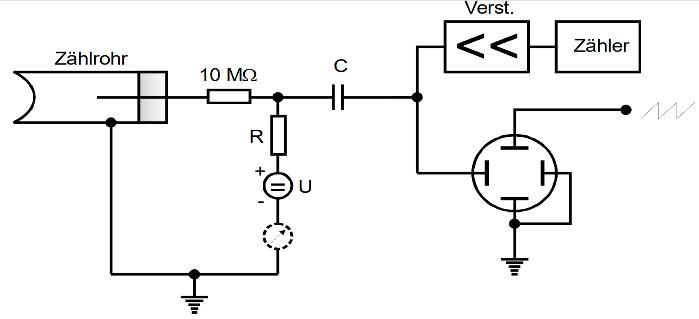
\includegraphics[scale=0.5]{content/images/aufbau2.jpg}
\caption{Versuchsaufbau zur Bestimmung der Kenndaten eines Geiger-Müller-Zählrohrs \cite{V703}.}
\label{fig:Aufbau}
\end{figure}